%!TEX root = ../main.tex

%------------------------------
%  Do not add notation macros to this file 
%  use notation.tex instead
%-------------------------------

%----- Theorems ----------------------------------------------------------------
%\newtheorem{theorem}{Theorem}
%\newtheorem{lemma}{Lemma}
%\newtheorem{corollary}{Corollary}
%\newtheorem{definition}{Definition}
%\newtheorem{example}{Example}
%\spnewtheorem*{definition*}{Definition}{\bfseries}{\itshape}

\spnewtheorem*{theorem*}{Theorem}{\bfseries}{\itshape}
\spnewtheorem*{theoremnn}{Theorem}{\bfseries}{\itshape}
\spnewtheorem*{lemma*}{Lemma}{\bfseries}{\itshape}
\newenvironment{claimproof}[1]{\par\noindent\underline{Proof}:\space#1}{\hfill $\blacksquare$}

\newcommand{\ignore}[1]{\relax} 

%-------------------------------------------------------------------------------
%  Magic Stuff below
%-------------------------------------------------------------------------------

%------ Quote ------------------------------------------------------------------

\renewcommand{\quote}{\list{}{\rightmargin=\leftmargin\topsep=0pt}\item\relax}

%------ List Definitions -------------------------------------------------------
\newlength{\saveparindent}
\setlength{\saveparindent}{\parindent}
\newlength{\saveparskip}
\setlength{\saveparskip}{\parskip}
\newcounter{ctr}

\newenvironment{tiret}{%
\begin{list}{\hspace{1pt}\rule[0.5ex]{6pt}{1pt}\hfill}{\labelwidth=15pt%
\labelsep=3pt \leftmargin=18pt \topsep=1pt%
\setlength{\listparindent}{\saveparindent}%
\setlength{\parsep}{\saveparskip}%
\setlength{\itemsep}{1pt}}}{\end{list}}

\newenvironment{newenum}{%
\begin{list}{{\rm \arabic{ctr}.}\hfill}{\usecounter{ctr}\labelwidth=17pt%
\labelsep=6pt \leftmargin=23pt \topsep=.5pt%
\setlength{\listparindent}{\saveparindent}%
\setlength{\parsep}{\saveparskip}%
\setlength{\itemsep}{5pt} }}{\end{list}}

%------ Subsection and Paragraph -----------------------------------------------

\makeatletter
%\renewcommand{\section}{\abovedisplayskip 3\p@ \@plus3\p@ \@minus1\p@%
%                      \belowdisplayskip 5\p@ \@plus3\p@ \@minus1\p@%
%                      \abovedisplayshortskip 0pt \@plus2\p@%
%                      \belowdisplayshortskip 0pt \@plus2\p@ \@minus0\p@%
%                      \@startsection{section}{1}{\z@}%
%                       {-10\p@ \@plus -4\p@ \@minus -4\p@}%
%                       {6\p@ \@plus 4\p@ \@minus 4\p@}%
%                       {\normalfont\large\bfseries\boldmath
%                        \rightskip=\z@ \@plus 8em\pretolerance=10000 }}
%\renewcommand{\subsection}{\@startsection{subsection}{2}{\z@}%
%                      {-6\p@ \@plus -4\p@ \@minus -4\p@}%
%                      {2\p@ \@plus 2\p@ \@minus 2\p@}%
%                      {\normalfont\normalsize\bfseries\boldmath
%                       \rightskip=\z@ \@plus 8em\pretolerance=10000 }}
\renewcommand{\subsubsection}{\@startsection{paragraph}{4}{\z@}%
                      {-8\p@ \@plus -4\p@ \@minus -4\p@}%
                      {-5\p@ \@plus -0.22em \@minus -0.1em}%
                      {\normalfont\normalsize\bfseries\boldmath
                      }}
%\renewcommand{\paragraph}[1]{\medskip\noindent{\bf #1}}
\renewcommand{\paragraph}{\@startsection{paragraph}{4}{\z@}%
                      {-8\p@ \@plus -4\p@ \@minus -4\p@}%
                      {-5\p@ \@plus -0.22em \@minus -0.1em}%
                      {\normalfont\normalsize\bf
                      }}
\makeatother

%----- Comments ----------------------------------------------------------------
\RequirePackage{totcount}
\RequirePackage{color}
\RequirePackage[colorinlistoftodos]{todonotes}

\newtotcounter{notecount}
\newcommand{\notewarning}{%
\ifnum\totvalue{notecount}>0%
 \vspace{1ex}
\begin{center}
 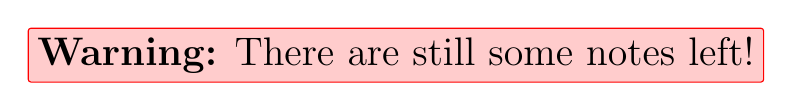
\begin{tikzpicture}[baseline=(A.south)]
    \node (A) [] at (0,0){};
    \node [rounded corners=1pt,rectangle, draw=red, fill=red!20,text=black](B) at (0.1ex,0ex){
        \Large \raggedright {\bf Warning:} There are still some notes left!
    };
 \end{tikzpicture}
\end{center}
 \vspace{1ex}
\fi
}
\makeatletter
\def\myaddcontentsline#1#2#3{%
  \addtocontents{#1}{\protect\contentsline{#2}{#3}{Section \thesubsection\ at p. \thepage}{}}}
\renewcommand{\@todonotes@addElementToListOfTodos}{%
    \if@todonotes@colorinlistoftodos%
        \myaddcontentsline{tdo}{todo}{{%
            \colorbox{\@todonotes@currentbackgroundcolor}%
                {\textcolor{\@todonotes@currentbackgroundcolor}{o}}%
            \ \@todonotes@caption}}%
    \else%
        \myaddcontentsline{tdo}{todo}{{\@todonotes@caption}}%
   \fi}%
\newcommand*\mylistoftodos{%
  \begingroup
       \setbox\@tempboxa\hbox{Section 9.9 at p. 99}%
       \renewcommand*\@tocrmarg{\the\wd\@tempboxa}%
       \renewcommand*\@pnumwidth{\the\wd\@tempboxa}%
       \listoftodos%
  \endgroup
}
\makeatother
\definecolor{lightgreen}{rgb}{0.86, 0.93, 0.78}
\definecolor{bordergreen}{rgb}{0.55, 0.76, 0.74}
\definecolor{lightblue}{rgb}{0.70, 0.90, 0.99}
\definecolor{borderblue}{rgb}{0.01, 0.66, 0.96}
\definecolor{lightamber}{rgb}{1, 0.93, 0.70}
\definecolor{borderamber}{rgb}{1, 0.76, 0.03}
\definecolor{lightcolor4}{rgb}{ 0.93, 0.70, 1}
\definecolor{bordercolor4}{rgb}{0.76, 0.03, 1}
\newcommand{\pnote}[1]{\stepcounter{notecount}\todo[inline,bordercolor=bordergreen,linecolor=bordergreen,color=lightgreen]{\footnotesize{\sc \bf Peter:} #1}{}}
\newcommand{\cnote}[1]{\stepcounter{notecount}\todo[inline,bordercolor=borderblue,linecolor=borderblue,color=lightblue]{\footnotesize{\sc \bf Christian:} #1}{}}
\newcommand{\vnote}[1]{\stepcounter{notecount}\todo[inline,bordercolor=borderamber,linecolor=borderamber,color=lightamber]{\footnotesize{\sc \bf Vassilis:} #1}{}}
\newcommand{\myvnote}[1]{{\color{red}{\sc \bf Vassilis:} #1}\ \newline}
\newcommand{\anote}[1]{\stepcounter{notecount}\todo[inline,bordercolor=bordercolor4,linecolor=bordercolor4,color=lightcolor4]{\footnotesize{\sc \bf Aggelos:} #1}{}}

\newcommand{\TODO}[1]{
  \if\relax\detokenize{#1}\relax
    \textcolor{red}{TODO} 
  \else
    \textcolor{red}{ {#1}} 
  \fi
}

\newcommand{\footTODO}[1]{\footnote{\TODO{#1}}}


\newcommand{\pnotelite}[1]{
  \textcolor{blue}{\textbf{Peter: } {#1}} 
}

%----- Algorithm Environment ---------------------------------------------------
%Header for Algorithms/Functionalities
\newcommand{\algoHead}[1]{\vspace{0.2em} \underline{\textbf{#1}} \vspace{0.3em}}
\newcommand{\algoHeadExt}[2]{\vspace{0.2em} \underline{\textbf{#1} #2} \vspace{0.3em}}

%Multiline Algo-States
\makeatletter
\algnewcommand{\ExtendedState}[1]{\State
\parbox[t]{\dimexpr\linewidth-\ALG@thistlm}{\hangindent=\algorithmicindent\strut\hangafter=3#1\strut}}
\makeatother

%Algorithms States
\algnewcommand\algorithmicinput{\textbf{Input:}}
\algnewcommand\Input{\item[\algorithmicinput]}
\renewcommand{\algorithmicensure}{\textbf{Output:}}

%Algo Comments
\algrenewcommand{\algorithmiccomment}[1]{{\color{gray}// #1}}

%----- Box Environment ---------------------------------------------------------
\RequirePackage{mdframed}

%Basic box structure with title box
\newenvironment{titlebox}[3]
 {\mdfsetup{
   style=#2,
   innertopmargin=1.1\baselineskip,
   skipabove={\dimexpr0.7\baselineskip+\topskip\relax},
   skipbelow={1em},needspace=3\baselineskip,
   singleextra={\node[#3,right=10pt,overlay] at (P-|O){~{\sffamily\bfseries #1 }};},%
   firstextra={\node[#3,right=10pt,overlay] at (P-|O) {~{\sffamily\bfseries #1 }};},
   frametitleaboveskip=9em,
   innerrightmargin=5pt
  }
  \begin{mdframed}[font=\small]\setlist[itemize]{leftmargin=13pt}\setlist[enumerate]{leftmargin=13pt}\raggedright% 
 }
 {\end{mdframed}}

 %title box style
 \tikzstyle{normal} = [thick, fill=white, text=black, draw, rounded corners, rectangle, minimum height=.7cm, inner sep=3pt]
 \tikzstyle{gray} = [thick, fill=gray!90, text=white, rounded corners, rectangle, minimum height=.7cm, inner sep=3pt]

 %box style
 \mdfdefinestyle{commonbox}{%
  align=center, middlelinewidth=1.1pt,userdefinedwidth=\linewidth
  innerrightmargin=0pt,innerleftmargin=5pt,innertopmargin=5pt,
  splittopskip=15pt,splitbottomskip=15pt
 }
 \mdfdefinestyle{roundbox}{style=commonbox,roundcorner=5pt,userdefinedwidth=\linewidth}

 \newenvironment{systembox}[1]
 {\vspace{\baselineskip}\begin{titlebox}{Functionality \normalfont #1}{roundbox}{normal}}
 {\end{titlebox}}

 \newenvironment{gsystembox}[1]
 {\vspace{\baselineskip}\begin{titlebox}{Global Functionality \normalfont #1}{roundbox}{normal}}
 {\end{titlebox}}

 \newenvironment{protocolbox}[1]
 {\begin{titlebox}{Protocol \normalfont #1}{commonbox}{normal}}
 {\end{titlebox}}

 \newenvironment{algobox}[1]
 {\begin{titlebox}{Algorithm \normalfont #1}{commonbox}{normal}}
 {\end{titlebox}}

 \newenvironment{reductionbox}[1]
 {\begin{titlebox}{Reduction \normalfont #1}{commonbox}{normal}}
 {\end{titlebox}}

 \newenvironment{gamebox}[1]
 {\begin{titlebox}{Game \normalfont #1}{commonbox}{gray}}
 {\end{titlebox}}

 \newenvironment{simulatorbox}[1]
 {\begin{titlebox}{Simulator \normalfont #1}{commonbox}{normal}}
 {\end{titlebox}}

%----- Old macros --------------------------------------------------------------
%For old macros
\newcommand{\deprecated}[1][\relax]{%
 \begin{tikzpicture}[baseline=(A.south)]
    \node (A) [] at (0,0){};
    \node [rectangle, draw, fill=red!20,text=black](B) at (0.1ex,0ex){
        \raggedright DO NOT USE! 
        \if #1\relax\else
         Use instead: #1
        \fi
    };
 \end{tikzpicture}
}


%----- Reference magic ---------------------------------------------------------
%Enable reference of descriptions
\makeatletter
\let\orgdescriptionlabel\descriptionlabel
\renewcommand*{\descriptionlabel}[1]{%
  \let\orglabel\label
  \let\label\@gobble
  \phantomsection
  \edef\@currentlabel{#1}%
  %\edef\@currentlabelname{#1}%
  \let\label\orglabel
  \orgdescriptionlabel{#1}%
}
\makeatother


%----- Detect Texas Rangers ----------------------------------------------------
%\makeatletter
%\@namedef{tz-05}{`Texas Ranger'}
%\@namedef{tz-06}{`Texas Ranger'}
%\@namedef{tz-07}{`Texas Ranger'}
%\@namedef{tz+02}{`Texas Ranger'} 
%\def\grabtimezone #1#2#3#4#5#6#7#8#9{\grabtimezoneB}
%\def\grabtimezoneB #1#2#3#4#5#6#7{\grabtimezoneC}
%\def\grabtimezoneC #1#2'#3'{%
%  \@ifundefined{tz#1#2}
%    {}%If not in Texas Time Zone hide designation
%    {{\bf\@nameuse{tz#1#2}}\xspace}%
%}
%\def\texasranger{\expandafter\grabtimezone\pdfcreationdate}
%\stepcounter{notecount}
%\makeatother

%----- Restate Theorems ----------------------------------------------------


%environment for custom theorem numbers
\newtheorem{innercustomthm}{Theorem}
\newenvironment{customthm}[1]
{\renewcommand\theinnercustomthm{#1}\innercustomthm}
{\endinnercustomthm}

% legacy Praos macros
\newcommand{\mc}{\mathcal}
\newcommand{\vrflengthout}{\vrfoutlen}

